\section{O Sistema de Locomoção}
\subsection{Duto de Propulsão}
A água que é ejetada do sistema de filtragem é devolvida para a piscina, auxiliando assim a limpeza geral de todo o volume em que o robô está submerso. A água filtrada é direcionada para uma saída que se localiza na parte superior do produto. O duto de saída será um bocal direcionável localizado na parte superior do robô responsável por sua locomoção. Esse bocal irá se mover nas 4 direções principais, isto é, nos ângulos de 0, 90, 180 e 270 graus, proporcionando ao robô a locomoção necessária para o cumprimento da rota de limpeza.

O duto de propulsão terá diametro de 1” (25,4mm). Acoplado a ele está o propulsor auxiliar que permitirá a movimentação do robô com a velocidade desejada. O duto de propulsão foi construído de forma que a água mude de direção sem que haja vazamentos e que o servo responsável pela rotação não entre em contato com a água.

\subsection{As Rodas}
O aparelho contará com quatro rodas. Elas se assemelham as usadas em carrinhos de supermercado, com liberdade de 360 graus em relação ao eixo $x$ e $y$.
\par
  \begin{figure}[h]
    \centering
    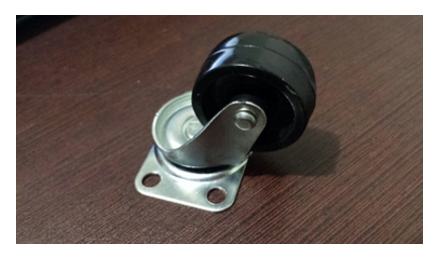
\includegraphics[width=0.6\textwidth]{figures/wheel-market.png}
    \caption{Rodas utilizadas para a locomoção do robô.}
    \label{fig:wheel-market}
  \end{figure}
  \FloatBarrier
\par
As rodas serão fixadas na placa da base do robô e estarão localizadas nos cantos da base do robô e direcionarão o seu movimento de acordo com a direção do jato de água oriundo do bocal, conforme a Figura \ref{fig:catia-base}.
\par
  \begin{figure}[h]
    \centering
    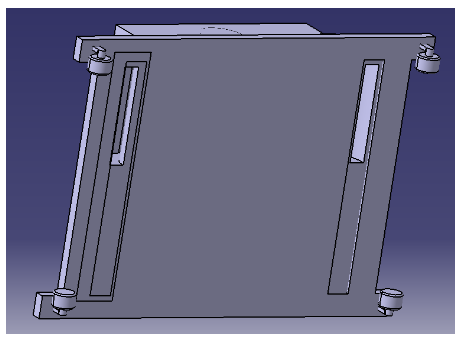
\includegraphics[width=0.8\textwidth]{figures/catia-base.png}
    \caption{Desenho da base do robô indicando as posições das rodas.}
    \label{fig:catia-base}
  \end{figure}
  \FloatBarrier
\par
